%%% TeX-command-extra-options: "--output-directory=build"
\documentclass{amsart}
\usepackage[margin=1in]{geometry}
\usepackage{afterpage}
\usepackage{tikz}
\usepackage{mathptmx}
\usetikzlibrary{fadings}
\usepackage{background}
\backgroundsetup{
scale=1,
angle=0,
opacity=0.6,  %% adjust
contents={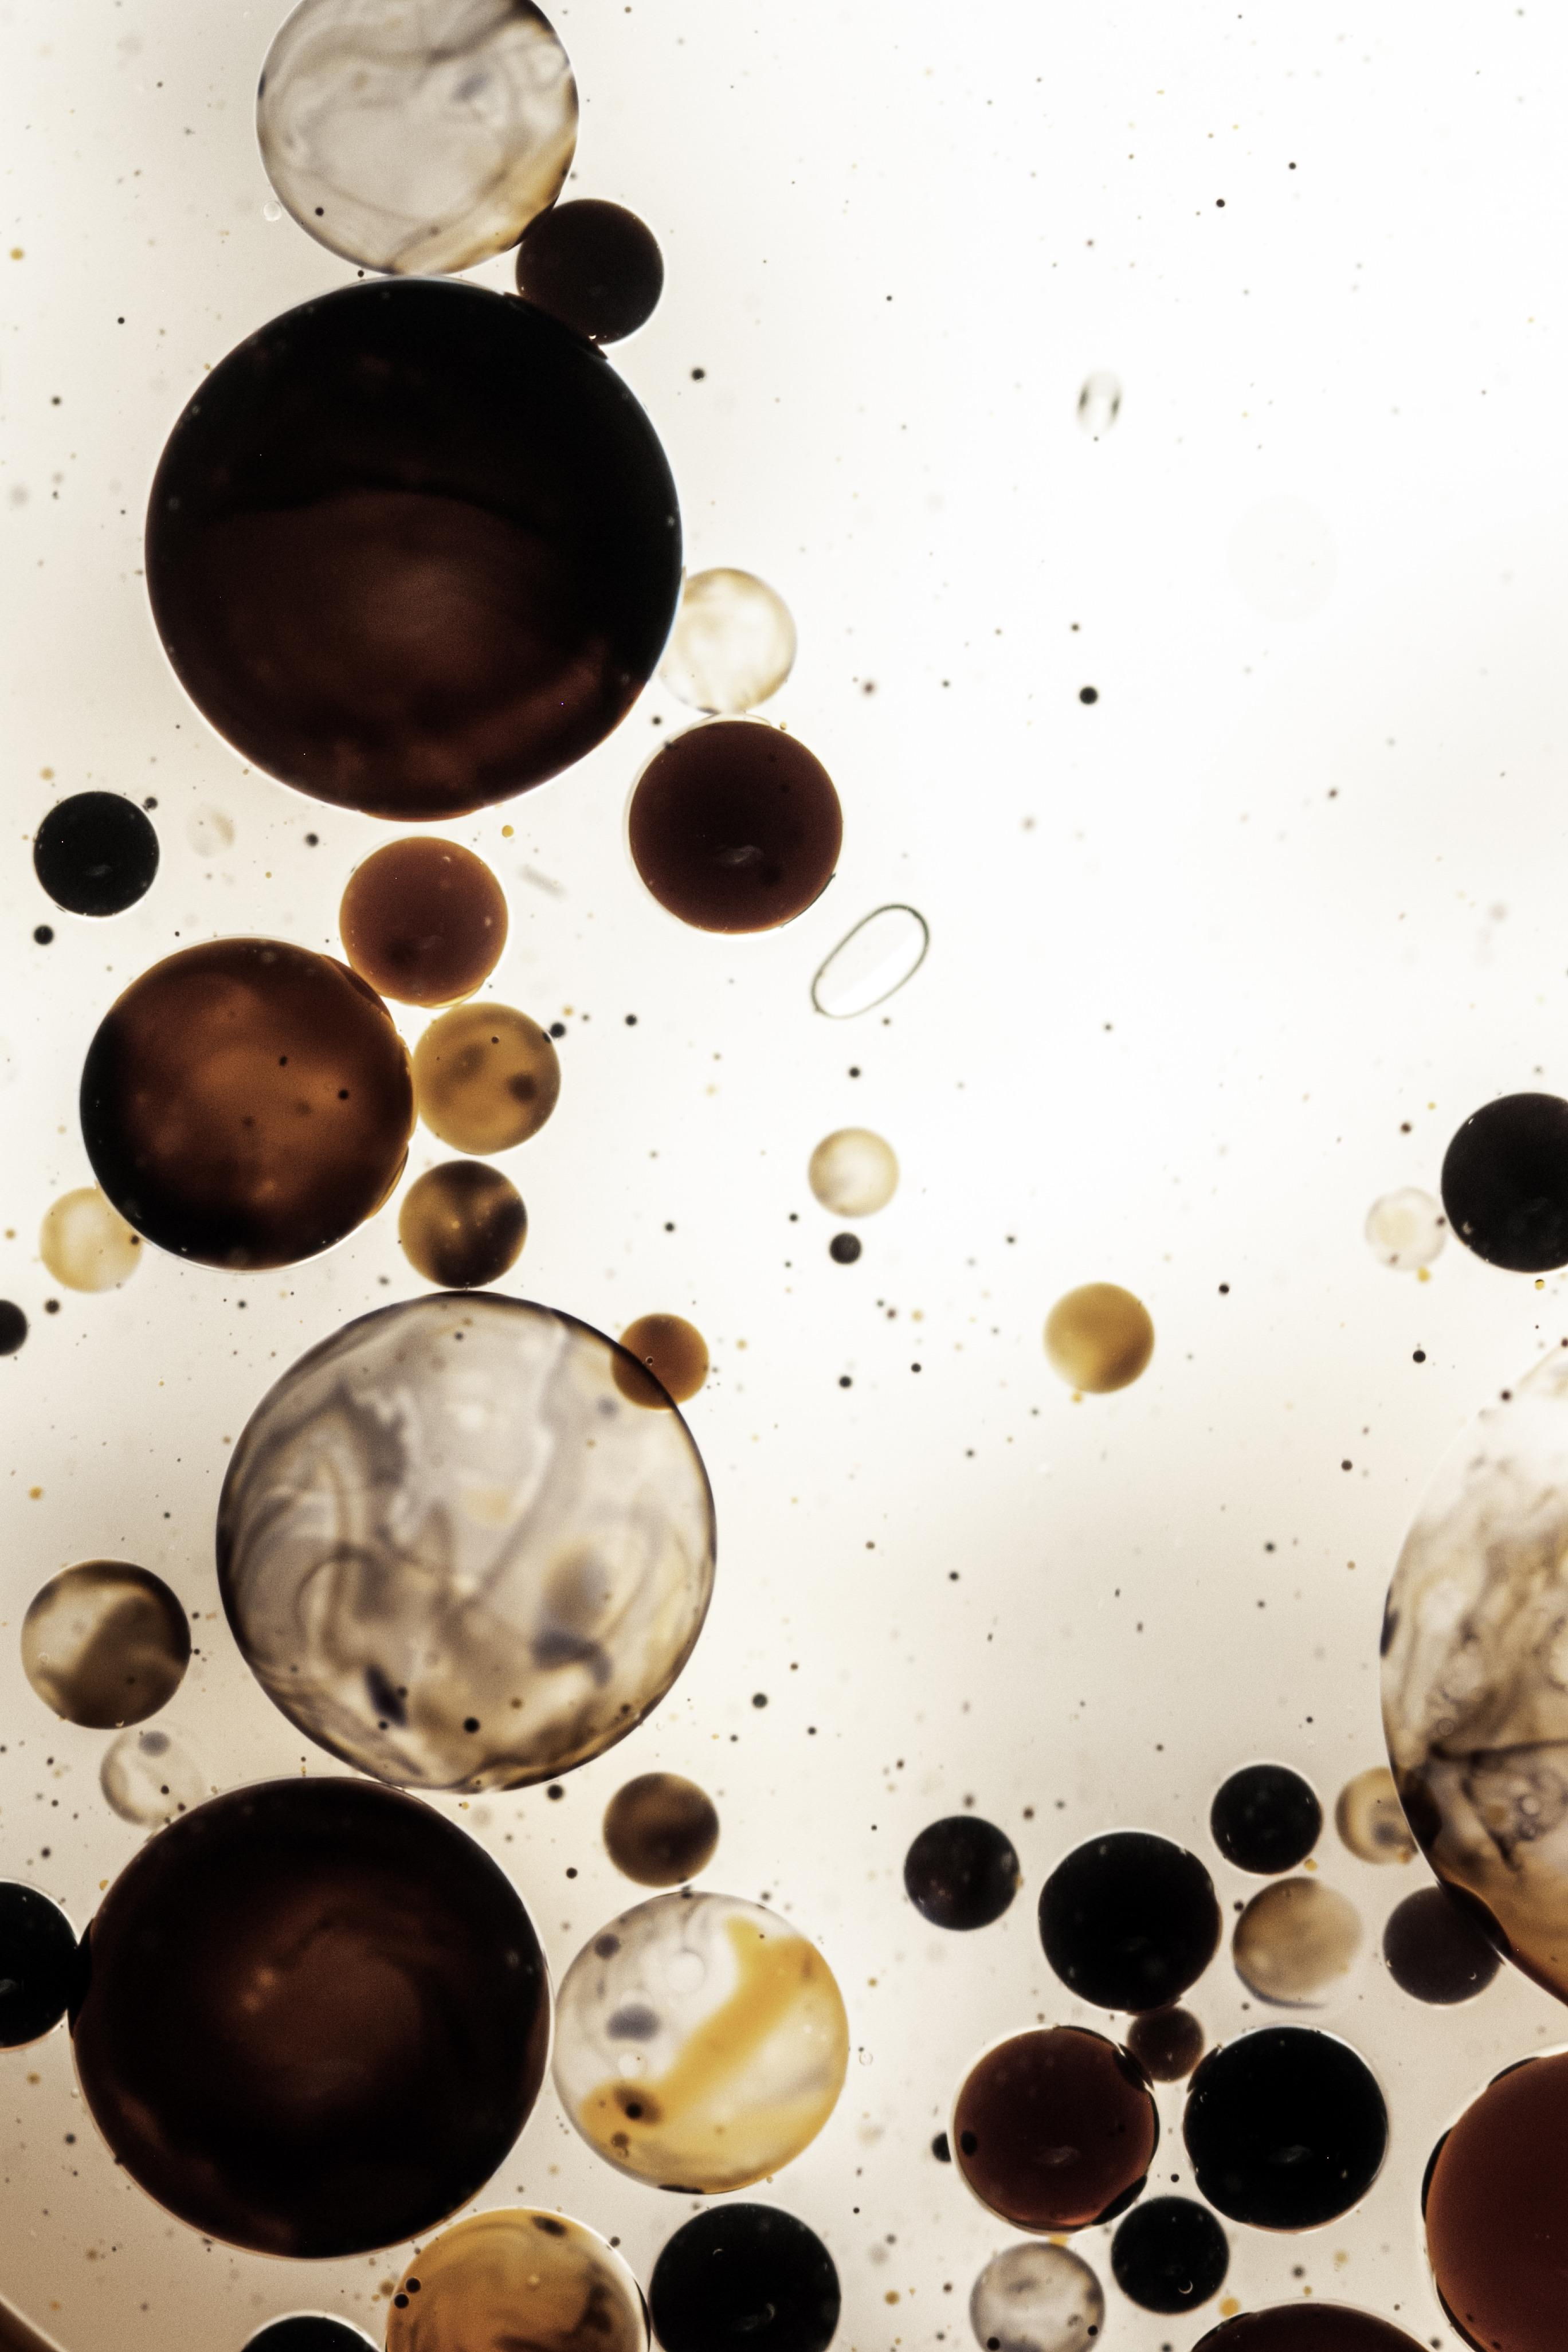
\includegraphics[width=\paperwidth,height=\paperheight]{coffee_bubbles.jpg}}
}

\begin{document}

\vspace*{\fill}

\begin{flushleft}
\Huge{\textbf{Why didn't anybody do this yet?}}
  
\LARGE{an okay summary of undergrad analog-based electrical engineering}

\vspace{0.2cm}
\Large{Garek Dyszel}
\end{flushleft}

\vspace*{\fill}

\tiny{Image credit: JustSlipAway at https://i.redd.it/pxgbyghuv1d51.jpg}

\end{document}
